\chapter{La mémoire}

%% \begin{itemize}
%% \item un article sur l'effet du cache sur les performances \url{http://igoro.com/archive/gallery-of-processor-cache-effects/}
%% \item \url{http://www.hardwaresecrets.com/how-the-cache-memory-works/7/}
%% \end{itemize}


Dans cette partie, on revient sur un composant : la mémoire. Jusque maintenant on ne s'est pas trop soucié de la question de la taille de la mémoire, du temps d'accès aux informations mémorisées, etc... et l'objet de ce chapitre est de se confronter à cette question. Dans une première partie, je vous propose une revue de différentes technologies pour réaliser des mémoires. Ce faisant, on verra qu'on ne dispose pas d'une technologie qui permette de réaliser des mémoires rapides, à faible coût et de grande capacité et on s'intéressera aux solutions techniques pour en donner malgré tout l'illusion avec notamment les mémoires caches. Il existe un autre mécanisme que nous n'aborderons pas dans ce cours qu'est la mémoire virtuelle qui est prise en charge logiciellement par le système d'exploitation.

\section{Les différentes formes de mémoire}

\subsection{Mémoire morte (ROM)}

On a l'habitude de regrouper sous l'appellation mémoire morte, des mémoires non volalites (le contenu n'est pas perdu même si l'alimentation est coupée) facilement accessible en lecture mais dont le contenu ne peut pas être modifié (ou difficilement) si la puce est insérée dans l'ordinateur, d'o{\`u} le terme anglais \emph{read-only memory} (ROM). 


En toute rigueur, une mémoire morte est une mémoire en lecture seule et donc forcément non volatile. Parfois, ce terme est utilisé de manière plus générale pour désigner les mémoires non volatiles. Mais la non volatilité n'implique pas forcément l'accès en lecture seule et il existe des mémoires non volatiles accessibles en lecture/écriture.

L'intérêt des mémoires non volatiles, comme leur nom l'indique, c'est qu'elles conservent leur contenu même en l'absence d'alimentation électrique. Une solution très simple pour réaliser une mémoire non volatile est de construire un circuit dont le contenu est écrit en détruisant des fusibles comme dans une PROM. Ces mémoires ne sont donc programmables qu'une fois et elles ne nécessitent pas d'alimentation pour mémoriser leur contenu. D'autres technologies comme les EPROM, EEPROM, permettent de modifier (un nombre de fois limité) le contenu et sont effaçables par exposition ultraviolette ou électriquement.

L'une des utilisations des ROM est de stocker quelques petits programmes pour le démarrage de l'ordinateur, notamment le SETUP et le BIOS (Basic Input Output System). Le but de ces programmes est essentiellement d'initialiser et de paramétrer des périphériques d'entrée/sortie (e.g. modifier la fréquence d'horloge du processeur, activer/désactiver certaines périphériques) et de passer ensuite le relais à un programme qui se trouve par exemple sur une clé USB ou un disque dur pour démarrer un système d'exploitation comme Windows, Linux, ... L'ordre dans lequel considérer les périphériques pour démarrer un système d'exploitation est paramétrable dans le BIOS. Puisque le BIOS et le SETUP sont paramétrables, et qu'il faut sauvegarder ces paramètres, ils n'utilisent pas qu'une ROM et sont accompagnés d'une mémoire en lecture/écriture qui est en général une petite mémoire consommant peu et alimentée par une petite pile.


%Les mémoires ROM coûtent moins cher à réaliser que les puces accessibles en lecture/écriture, ont des temps d'accès assez rapide et sont peu encombrantes.

\subsection{Mémoire vive (RAM)}
\subsubsection{Registres}

Lors du chapitre sur la logique séquentielle, nous avions introduit un composant mémoire, le registre, construit à partir de bascules, elles mêmes construites à partir de quelques transistors et dont je vous rappelle la construction sur la figure \ref{fig:mem_register}.

\begin{figure}[htbp]
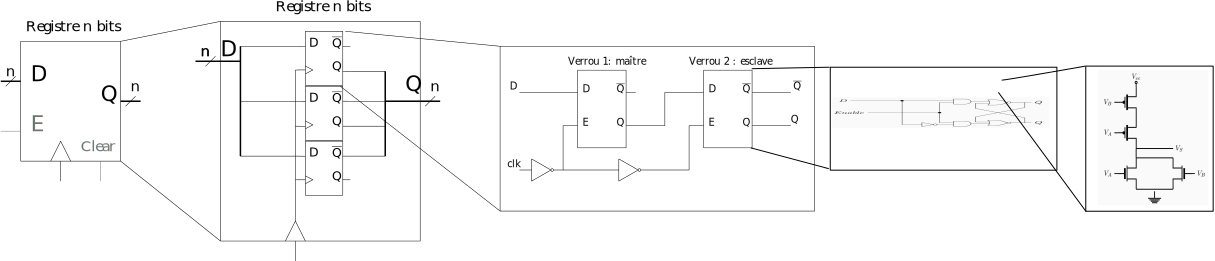
\includegraphics[width=\linewidth]{Figs/memory_register.pdf}
\caption{\label{fig:mem_register} Construction d'un registre à partir de bascules, elles-mêmes construites à partir de plusieurs transistors MOSFET.}
\end{figure}

Les circuits mémoires ainsi construit sont accessibles en lecture et écriture et sont dits volatiles : si l'alimentation est éteinte, les informations mémorisées sont perdues. Les temps d'accès sont en général de quelques pico-secondes ($10^{-12}s$) et ces registres ont des capacités de moins d'une centaine de bits (32 bits ou 64 bits par exemple).

\subsubsection{Static Random Access Memory (SRAM)}

Les mémoires statiques (SRAM) sont construites à partir d'éléments bistables, sur le même principe que les registres, mais avec un nombre plus limité de transistors\footnote{un registre a peut être besoin d'une dizaine ou vingtaine de transistors}. La figure \ref{fig:mem_sram} illustre une cellule mémoire d'un bit construite à partir de seulement 6 transistors MOSFET.

\begin{figure}[htbp]
\centering\includegraphics[width=0.5\linewidth]{Figs/sram_inner.pdf}
\caption{\label{fig:mem_sram} Une cellule d'un bit SRAM est construire à partir de deux inverseurs et deux transistors supplémentaires, soit 6 transistors MOSFET. }
\end{figure}

Le circuit n'admet que deux états stables $(Q, \overline{Q}) = (0,1)$ et $(Q, \overline{Q}) = (1, 0)$ qui permettent d'encoder les deux états binaires $0$ et $1$. Pour lire le contenu de la cellule, les deux transistors d'accès sont activés en appliquant une tension sur la ligne word line, de telle sorte que l'état $(Q, \overline{Q})$ est transmis sur les voies bit line. Ces signaux sont ensuite amplifiés et le bit mémorisé peut être lu.

Pour l'écriture, on commence par placer le bit à sauvegarder (et son complémentaire) sur les bit lines. On active ensuite les transistors d'accès. Le dimensionnement des transistors utilisés pour construire les inverseurs est tel que les niveaux logiques imposés sur les bit lines font dériver l'état $Q, \overline{Q}$ vers l'état à mémoriser.

Le fait que ce circuit utilise moins de transistors que les registres impliquent qu'il coûte moins chers et qu'il supporte une plus grande densité d'intégration (nombres de modules par cm$^2$), ce qui permet de construire des mémoires SRAM de plus grandes capacité (10 ko - 10 Mo) que les registres . Les mémoires construites à partir de ces cellules sont dites volatiles puisque l'information mémorisée est perdue si l'alimentation est coupée. Les temps d'accès sont de l'ordre de quelques ns ($10^{-9} s$). Ces mémoires sont utilisées pour construire ce qu'on appelle des caches (L1, L2, L3) et dont on va reparler bientôt.


\subsubsection{Dynamic Random Access Memory (DRAM)}

Les mémoires dynamiques DRAM reposent sur un principe différent des deux mémoires précédentes. Elles sont construites à partir d'un transistor et d'une capacité, comme illustré sur la figure \ref{fig:mem_dram}.

\begin{figure}[htbp]
\centering\includegraphics[width=0.2\linewidth]{Figs/dram_inner.pdf}
\caption{\label{fig:mem_dram} Une cellule d'un bit DRAM est construire à partir d'un transistor et d'une capacité. C'est le niveau de charge de la capacité qui détermine la valeur du bit mémorisée.}
\end{figure}
Pour écrire un bit, on place sur le bitline le niveau logique à mémoriser puis on active le transistor pendant un temps suffisant pour que la capacité se charge ou se décharge. Pour lire le bit mémorisé, on active la ligne word line, ce qui permet d'accéder au potentiel $V_c$ sur la bitline. La fermeture du circuit, causée par l'activation du transistor lors de la lecture, conduit à une perte de charge de la capacité et il est nécessaire, après chaque lecture, de réécrire l'état lu. Même si la donnée n'est pas accédée en lecture, la capacité a malgré tout tendance à perdre de la charge et dans tous les cas, il est nécessaire de rafraichir le contenu de la mémoire en faisant des réécritures régulières, environ une fois toutes les millisecondes. C'est pour cette raison que les mémoires construites sur ce type de cellule sont appelée dynamique.

Comme ces mémoires n'utilisent qu'un transistor et une capacité, elles supportent une plus grande densité d'intégration que les mémoires SRAM et ce sont d'ailleurs ces mémoires DRAM qui sont utilisées pour construire les mémoires principales. Le temps d'accès à ces mémoires est plus important que pour les SRAM notamment parce qu'il faut rafraîchir régulièrement son contenu.


\subsection{Mémoire de masse : disque dur}

Un disque dur est une mémoire de masse magnétique constituée de plusieurs plateaux, accédé en lecture et écriture grâce au déplacement mécanique de têtes de lecture. Sur chaque plateau, on trouve de l'ordre de quelques milliers de pistes, chacune divisée en secteur. Chaque secteur contient de l'ordre de 512 octets. Les technologies de disque dur autorise aujourd'hui des disques de plusieurs Go voire To ($2^{43}$ bits). Puisqu'il faut mettre en mouvement un système mécanique, les temps d'accès à une information sont considérablement plus long notamment que les mémoires présentées jusque maintenant. Les disques durs à $7400 tr/min$, i.e. $120 tr/s.$ mettent de l'ordre de la milliseconde pour faire une révolution. Par contre, les accès séquentiels, pour des informations proches de la tête de lecture sont assez rapide d'accès. Le disque dur est une mémoire de masse non volatile : les données ne sont pas perdues si l'alimentation est coupée.

\begin{figure}[htbp]
\centering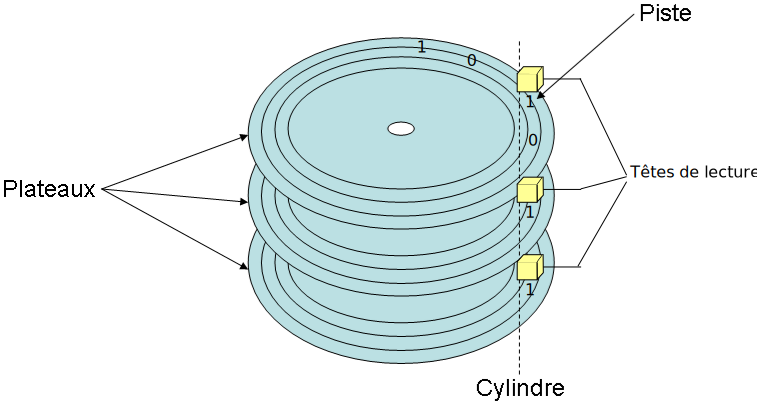
\includegraphics[width=0.5\linewidth]{Figs/dd.pdf}
\caption{\label{fig:mem_dd} Un disque dur est constitué de plusieurs plateaux, accédé en lecture ou en écriture en déplaçant mécaniquement des têtes de lecture. Image originale de wikipedia.org.}
\end{figure}

\subsection{Synthèse des mémoires en lecture/écriture : vive et de masse}

Les différentes technologies de mémoire sont comparables sur plusieurs critères. La \textbf{capacité} définit le nombre de bit qu'un module peut mémoriser\footnote{il faudrait plutôt utiliser la densité en bit/cm$^2$.}. La \textbf{latence} corresponds au temps qu'il faut attendre pour accéder à un module en lecture ou en écriture. Un dernier critère que nous allons considérer est le coût d'un module. Ces critères pour les différentes mémoires vives et mémoires de masse sont résumés dans le tableau \ref{table:memory_properties}.

%La bande passante corresponds au nombre de bits échangés par seconde avec le module mémoire qui dépends elle-même du nombre de bits échangés simultanément et de la latence.

\begin{table}[hbtp]
\centering\begin{tabular}{cccc}
Type & Capacité & Latence & Coût (au  Gi-octet) \\
\hline
Registre & 100 bits & 20 ps & très cher\\
SRAM & 10 Ko - 10 Mo & 1-10 ns & $\approx$ 1000 \euro\\
DRAM & 10 Go & 80 ns & $\approx$ 10 \euro\\
Flash & 100 Go & 100 $\mu s$& $\approx$ 1 \euro\\
Disque dur & 1 To & 10 ms & $\approx$ 0.1 \euro
\end{tabular}
\caption{\label{table:memory_properties} Capacité, latence et coût de différentes technologies de mémoires accessibles en lecture/écriture.}
\end{table}


On a donc fondamentalement un problème à résoudre. On ne peut apparemment pas disposer d'une mémoire qui soit à la fois rapide et de grande capacité. L'introduction du principe des mémoires cache, présenté dans les prochaines parties, nous permet justement de résoudre ce problème.

\section{Hierarchie de mémoire}
\subsection{Principe de localité spatiale et temporelle}

Lorsqu'on a déroulé l'exécution d'un programme dans les chapitres précédents, on a vu qu'on a tendance à accéder à des instructions et des données qui sont proches l'une de l'autre en mémoire : en général, on accède à des mots mémoires consécutifs quand on déroule un programme, ce qu'on appelle la \textbf{localité spatiale}. Souvent, il arrive également qu'on ai besoin d'accéder au même mot mémoire pendant quelques temps (comme lorsqu'on exécute des boucles), ce qu'on appelle la \textbf{localité temporelle}. Pour mieux se représenter ces principes de localité spatiale et temporelle, la figure \ref{fig:localite} illustre ce que pourrait être des accès mémoire pendant le déroulement d'un programme. Ce sont ces formes particulières qui donnent naissance au principe de localité et c'est ce qui est exploité pour construire des mémoires rapides et de grande capacité.

\begin{figure}[htbp]
\centering\includegraphics[width=0.5\linewidth]{Figs/localite.pdf}
\caption{\label{fig:localite} Principe de localité. Lors de l'exécution d'un programme, la mémoire est accédée à des adresses contiguës pour les instructions et opérandes (localité spatiale). Par ailleurs, il arrive fréquemment qu'une même variable ait besoin d'être accédée de manière répétée dans un petit laps de temps (localité temporelle). Chaque point représente une adresse mémoire accédée.}
\end{figure}


\subsection{Structure hierarchique de la mémoire: le meilleur des deux mondes}

Pour exploiter le principe de localité, on peut suivre deux approches. Une première consiste à disposer plusieurs modules mémoires de capacité et temps d'accès variables et de laisser le soin au programmeur d'utiliser l'une ou l'autre des mémoires. Si par exemple le programmeur sait qu'il a besoin d'accéder à un mot mémoire de manière répétée, il pourrait la charger dans une mémoire rapide le temps de l'utiliser puis la transférer dans une mémoire de plus grande capacité pour libérer de la place dans la petite mémoire rapide. Ca n'est évidemment pas très confortable pour le développeur et il serait préférable d'automatiser ces transferts.

\begin{figure}[htbp]
\includegraphics[width=\linewidth]{Figs/cache_mem}
\caption{\label{fig:cache_mem} La mémoire est construite de manière hiérarchique avec des manières rapides mais de faible capacité proche du processeur et des mémoires plus lentes mais de plus grande capacité en s'en éloignant.}
\end{figure}

Une autre solution, beaucoup plus confortable pour le programmeur, est de construire une chaîne de mémoire en mettant des mémoires de plus en plus rapide mais de moins en moins grosse en se rapprochant du processeur, comme illustré sur la figure \ref{fig:cache_mem} avec le processeur, la mémoire principale (DRAM) et au milieu une petite mémoire rapide (SRAM) appelée mémoire cache. Le principe est alors que lorsqu'on accède à un mot mémoire, si il est présent en cache (on parle de \textbf{cache hit}) il est retourné rapidement au processeur et si il est absent (on parle de \textbf{cache miss}), il est demandé au module mémoire suivant. Pour mesurer les performances de ce type de configuration, on introduit deux grandeurs calculées à partir du nombre de hits et de misses :
\begin{itemize}
\item le hit ratio (HR) est le nombre d'accès pour lesquels le mot était en cache : HR = hits / (hits + misses)
\item le miss ratio (MR) est le nombre d'accès pour lesquels le mot n'était pas en cache : MR = misses/(hits + misses)
\end{itemize}
On peut alors calculer le temps moyen d'accès à un mot mémoire comme $T_m \approx HR. t_{cache} + MR t_{mem} = HR t_{cache} + (1 - HR) t_{mem}$. Avec par exemple, $t_{cache} = 10 ns, t_{mem} = 80 ns$, $T_m = 80 - 70 HR$. On sait aujourd'hui construire des caches pour lesquels $HR \approx 90 \%$, ce qui conduit à $T_m \approx 17 ns$. La gestion des caches se fait matériellement comme nous allons le voir dans les prochaines parties. Concernant les échanges entre la mémoire principale et les mémoires de masse, c'est le système d'exploitation qui les prends en charge avec un mécanisme qu'on appelle mémoire virtuelle et qu'on ne présentera pas dans ce cours.





%% \begin{itemize}
%% \item le cache prends en charge la localité temporelle : en mémorisant l'info dans el cache
%% \item le cache prends en charge la localité spatiale en important des blocs
%% \end{itemize}

%ex de la somme des premiers éléments d'un tableau accédé en séquence :  sum += a[i]; localité temprelle avec sum et localité spatiale en important tout le tableau. Ca c'est pour les données mais on peut aussi raisonner sur les instructions.


\section{Mémoire cache}

Le principe général d'un cache est qu'il est placé avant une mémoire plus grande mais plus lente et qu'il contient une sous-partie de celle-ci. Lorsqu'une requête d'accès lui est émise, il doit vérifier s'il dispose du mot mémoire demandé, si c'est le cas (cache hit) le retourner au processeur et sinon (cache miss) émettre la requête au niveau mémoire suivant. Dans les parties suivantes, on étudie plusieurs structures de cache.


%\subsection{Structure et terminologie}

%\todo{Schéma avec cpu - cache - mémoire principale}; cache hit et cache miss.
\subsection{Cache à correspondance directe}

Supposons qu'on dispose d'une mémoire principale adressable sur $n_a$ bits avec des mots de $n_d$ bits. Un cache direct est une mémoire adressable avec $n_c$ bits d'adresses et plusieurs champs :
\begin{itemize}
\item valid (1 bit) : est ce que la donnée est valide ? par exemple, tant qu'une ligne de cache n'a pas été chargée au moins une fois depuis la mémoire principale, elle est invalide
\item tag ($n_a - n_c$ bits) : bits de poids forts de l'adresse mémoire
\item data ($n_d$ bits) : le mot mémoire  
\end{itemize}

Lorsqu'un mot mémoire est demandé par le processeur, les $n_c$ bits de poids faibles sont utilisés pour adresser le cache. La figure \ref{fig:cache_direct} illustre le cas d'adresses mémoires et de mots de 16 bits, l'index étant les 4 bits de poids faibles. Notons ``index'' ces bits de poids faibles et cache[index] la ligne de cache correspondante. Si la ligne est valide et le tag corresponds aux bits de poids forts de l'adresse demandée, on a un hit et le mot mémoire stocké en cache est retourné au processeur. Par exemple, on aurait un cache hit si le processeur demandait l'adresse $0\times0041$, avec index=1 et tag=$0\times004$. Si jamais la ligne est invalide ou si le tag ne correspond pas, on a un miss. Par exemple, si le processeur demandait $0\times0200$ ou $0\times0042$ on aurait un cache miss.

\begin{figure}[htbp]
\includegraphics[width=\linewidth]{Figs/direct_cache.pdf}
\caption{\label{fig:cache_direct} Dans un cache direct, quelques bits de poids faible sont utilisés pour adresser le cache. Les bits de poids fort sont alors comparés au champ tag du cache. S'ils correspondent et si l'entrée est valide, on a un hit et la donnée est retournée. Sinon, on a un miss et le mot doit être demandé au niveau mémoire suivant.}
\end{figure}

Dans le cas d'un miss, il faut alors faire une demande du mot mémoire au niveau mémoire suivant. Lorsque le niveau mémoire suivant retourne le mot mémoire, celui-ci prends la place qui avait causé le miss. On parle de cache à correspondance directe puisqu'un mot mémoire ne peut se trouver qu'à une seule position dans le cache, celle indexée par ses bits de poids faible. On utilise les bits de poids faible pour respecter le principe de localité. En utilisant les bits de poids faible pour adresser le cache, on s'assure en effet que des adresses proches peuvent être stockées dans des lignes de cache différentes : des adresses proches ont des bits de poids faible différent; Par exemple, les adresses $0\times0100$, $0\times0101$, $0\times0102$ seraient stockées sur les premières lignes de cache. On peut aussi prendre en compte le principe de localité spatiale en mémorisant plusieurs mots mémoire par ligne de cache. Par exemple, on pourrait stocker sur chaque ligne de cache $4$ mots mémoires consécutifs. On décomposerait alors l'adresse mémoire en $12$ bits de tag, $2$ bits d'index et $2$ bits d'offset (fig.\ref{fig:cache_direct_block}). Le cache aurait alors 4 lignes de caches, chacune de 4 mots. En disposant d'un bus mémoire suffisamment large entre le cache et la mémoire principale, un échange entre le cache et la mémoire principale ramène dans ce cas 4 mots consécutifs. Pousser ce raisonnement à l'extrême, on pourrait penser qu'il suffit d'avoir une très grande ligne de cache. En pratique, à taille de cache constante, en augmentant la taille d'une ligne de cache, on diminue le nombre de lignes de cache et par là même, on diminue le nombre de régions de la mémoire qui peuvent être chargées simultanément. En pratique, on a malgré tout toujours besoin d'accéder à quelques régions distantes de la mémoire (\ref{fig:localite}).


\begin{figure}[htbp]
\includegraphics[width=\linewidth]{Figs/direct_cache_block.pdf}
\caption{\label{fig:cache_direct_block} En accord avec le principe de localité spatiale, les performances du cache sont améliorées si chaque ligne de cache héberge plusieurs mots consécutifs. }
\end{figure}

Le principal problème avec le cache à correspondance directe est que plusieurs adresses mémoires se projettent sur une même ligne de cache. Par exemple, si nos adresses sont codées sur 16 bits, et qu'on dispose d'un cache à $4$ bits d'adresses avec 1 mot par ligne de cache, les adresses 0x0101, 0x0201, 0x301 se projettent toutes sur la même ligne de cache. Si jamais notre programme\footnote{par exemple un programme dont les instructions commencent à l'adresse 0x0101 accédant à des variables stockées aux adresses 0x0201, 0x0202, ..} a besoin d'accéder de manière répétée aux mots mémoires aux adresses 0x0101, 0x0201 et 0x0301, on aura beaucoup de cache miss et donc des performances dégradées. Le problème fondamental étant que plusieurs mots mémoires ciblent les mêmes lignes de cache, il ``suffit'' de proposer une structure de cache dans laquelle chaque mot mémoire peut occuper n'importe quelle ligne de cache et c'est ce que proposent les caches associatifs.



%% \begin{itemize}
%% \item chaque mot mémoire ne se projette que sur une entrée de cache : d'ou le correspondance directe
%% \item ségmentation de l'adresse en index bit, tag bit ; les index bit sont pris sur les poids faibles pour répondre au principe de localité temporelle : les adresses proches peuvent être stockées à des adresses différentes en cache
%% \item on ajoute des bits d'offset pour ramener plusieurs blocs consécutifs, quelle taille de bloc ? avec un nombre constants de bits mémorisables, beaucoup de petits blocs ou peu de gros blocs
%% \item problème avec les caches direct : conflict misses avec des miss à répétition
%% \end{itemize}

\subsection{Cache associatif}

Dans un cache associatif, chaque mot mémoire peut occuper n'importe quelle ligne de cache. Avec un cache $N$ lignes, on dispose $N$ comparateurs (contre 1 seul pour le cache à correspondance directe, un multiplexeur étant utilisé pour diriger en entrée du comparateur le champ TAG associé à la ligne indexée par l'adresse demandée), comme illustré sur la figure \ref{fig:cache_associatif}. Lorsqu'un mot mémoire est demandé, les $N$ comparateurs effectuent en parallèle la comparaison entre l'adresse des mots en cache et l'adresse demandée. Si l'adresse se trouve en cache, les données sont directement retournées au processeur. 

\begin{figure}[htbp]
\centering\includegraphics[width=0.7\linewidth]{Figs/associatif_cache.pdf}
\caption{\label{fig:cache_associatif} Dans un cache associatif, chaque mot mémoire peut se trouver à n'importe quelle ligne de cache minimisant ainsi le risque que les adresses ayant les mêmes bits de poids faibles ne causent des caches miss. Les bits de poids fort de l'adresse demandée sont comparés en parallèle avec les adresses mémorisées dans le cache.}
\end{figure}

La gestion du cas o{\`u} l'adresse ne se trouve pas en cache est plus compliquée que pour le cache à correspondance directe. En effet, dans ce cas, il faut choisir une ligne de cache à laquelle placer les données qu'on va récupérer en mémoire, ce qu'on appelle une politique de remplacement. Une politique de remplacement possible\footnote{il existe une politique optimale, l'algorithme de Belady, qui consiste à supprimer la ligne de cache de l'adresse dont on aura besoin le plus tard, mais qui n'est pas utilisable en pratique justement à cause de l'incapacité de prédire, en général, l'utilisation à venir des adresses mémoires} est la politique \emph{Least Recently Used} (LRU) qui consiste à remplacer la ligne de cache la moins récemment utilisée. Cette politique prends donc en compte la manière dont le processeur utilise les données stockées en cache (en remplaçant plutôt une donnée qui n'est plus utilisée depuis longtemps qu'une donnée utilisée fréquemment) mais est coûteuse puisqu'elle nécessite de construire une liste ordonnée des accès aux lignes de cache.

\subsection{Cache associatif à n entrées}

Le cache à correspondance direct présente l'inconvénient que plusieurs mots mémoires entrent en compétition pour la même ligne de cache : si par exemple $12$ bits de poids forts sont utilisés pour le champ ``tag'' et 4 bits de poids faibles pour l'index et l'offset, toutes les adresses mémoires séparées de $2^4 = 16$ ciblent la même ligne de cache. Un cache associatif évite ce problème en autorisant n'importe quel mot mémoire à occuper n'importe quelle ligne de cache mais avec une complexité de réalisation considérable. Le cache associatif à n entrées est une forme hybride de ces deux caches. Dans un cache associatif à n entrées, on dispose d'un cache à correspondance direct dans lequel chaque ligne de cache est un cache associatif (fig.\ref{fig:cache_nway}). 

\begin{figure}[htbp]
\centering\includegraphics[width=\linewidth]{Figs/nway_cache.pdf}
\caption{\label{fig:cache_nway} Un cache associatif à n entrées est un cache à correspondance direct dans lequel chaque ligne de cache est un cache associatif. Cette réalisation permet d'alléger la complexité d'un cache associatif pur tout en évitant les conflits d'un cache à correspondance directe.}
\end{figure}

\subsection{Cohérence du cache et de la mémoire centrale}

Puisqu'un mot mémoire peut se trouver en cache et en mémoire principale, il se pose la question de la cohérence de ces deux mots d'une même adresse. Il existe plusieurs politiques pour assurer la cohérence des données en cache et des données en mémoires principales. Une première stratégie, la stratégie d'écriture immédiate (\emph{write through}) consiste à propager la modification du mot mémoire en cache en mémoire principale. Cela veut dire que chaque fois qu'un mot est écrit en cache, il sera aussi écrit en mémoire principale. Une deuxième stratégie, la stratégie à écriture différée (\emph{write back}), sollicite moins les échanges entre le cache et la mémoire principale. Elle consiste à n'écrire en mémoire principale une ligne de cache que lorsque celle ci est remplacée. On ajoute aussi un bit (\emph{dirty bit}) indiquant si la ligne a été modifiée pour s'éviter une copie en mémoire principale lors du remplacement de la ligne si jamais celle-ci n'a pas été modifiée.


%\section{Mémoire virtuelle}
